\documentclass[12pt]{article}


% Codificación de caracteres e idioma
\usepackage[utf8]{inputenc}
\usepackage[spanish]{babel}

% Tamaño de página y márgenes
\usepackage[letterpaper, margin=2.54cm]{geometry}

% Orientación horizontal de página
\usepackage{pdflscape}

% Comillas, columnas, gráficos, símbolos matemáticos e ingreso de código de programación
\usepackage{csquotes, multicol, graphicx, amssymb, amsmath, listings, xcolor}

% Para hacer mosaico de figuras
\usepackage{subcaption}

% Interlineado 1.5
\usepackage{setspace}
\onehalfspacing

% Uso de punto decimal, en lugar de coma
\decimalpoint

% Separación de columnas y sangría
\setlength{\columnsep}{2cm} 
\setlength{\parindent}{0cm}

% Páginado
\pagestyle{plain}

% Evitar separación de palabras
\hyphenpenalty=10000
\exhyphenpenalty=10000
\sloppy


\begin{document}

\begin{titlepage}
	\centering
	{\scshape\LARGE Universidad Aztlán \par}
	\vspace{1cm}
	{\scshape\Large Campus Playa del Carmen \par}
	\vspace{1.75cm}
	{\scshape\Huge Sistema de Gestión de una Tienda \par}
    \vfill
    {\itshape\Large Proyecto Final \par}
	\vspace{2cm}
    {\itshape\Large Presentado por: \par}
	{\Large José Rosendo Camal Teh \par}
	\vfill
	{\Large Ingeniería en Sistemas Computacionales \par}
	{\Large Cuarto Cuatrimestre \par}
	{\Large Fundamentos de Bases de Datos \par}
	\vfill
	{\Large Profe. Emmanuel Andrés Martínez López \par}
	\vfill
	{\Large 23 de octubre de 2026 \par}
	\vfill
	{\Large Playa del Carmen, Quintana Roo \par}
\end{titlepage}
\newpage


\tableofcontents

\newpage 

\section*{\centering Diagrama Entidad-Relación}
\addcontentsline{toc}{section}{Diagrama Entidad-Relación}
\vfill
\begin{figure}[htbp]
	\centering
	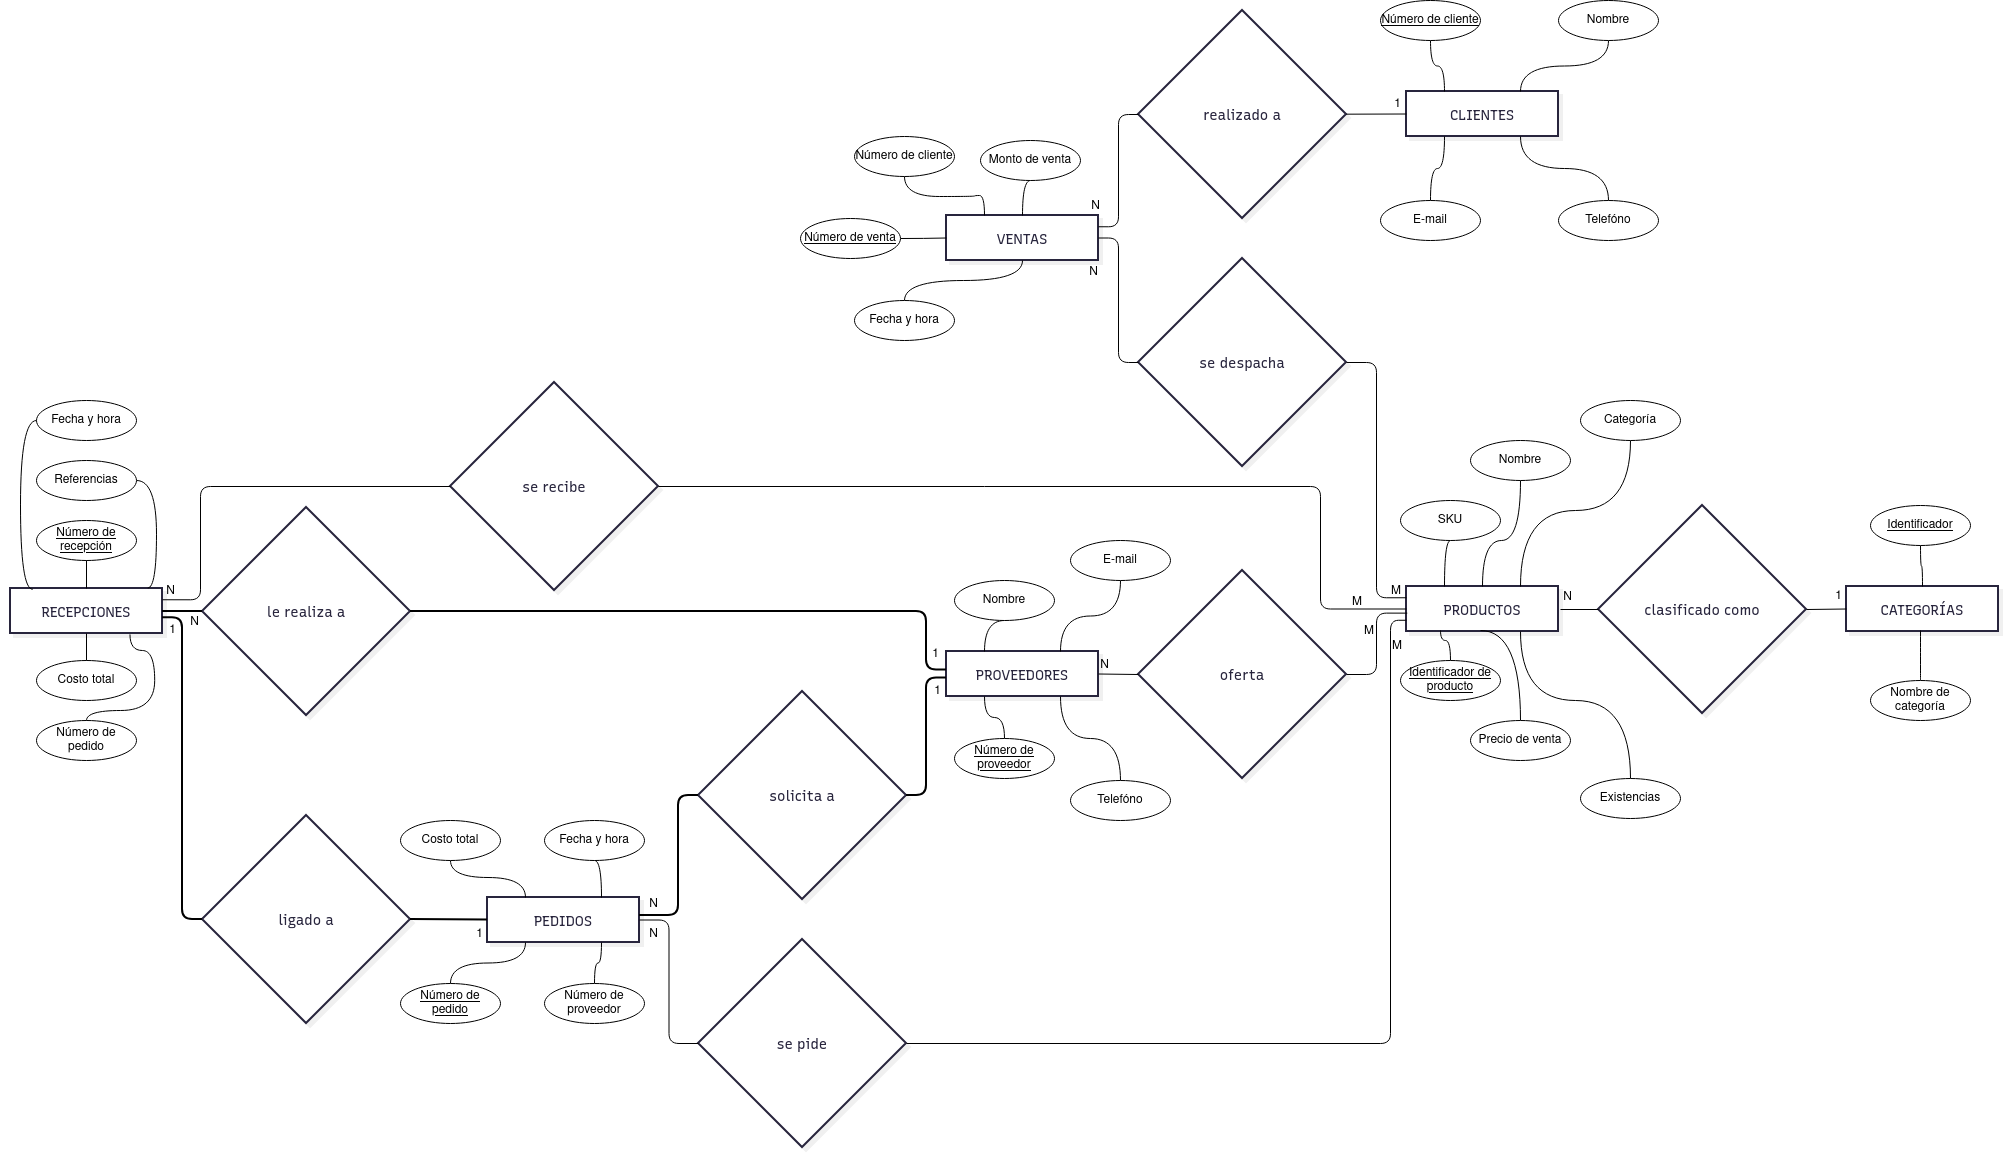
\includegraphics[
        width=0.7\textheight,
        height=0.7\textwidth,
        angle=-90
        ]{../img/erDiagram.drawio.png}
	\caption{Diagrama ER}
	\label{fig:erDiagram}
\end{figure}
\vfill
\newpage

\section*{\centering Modelo Relacional}
\addcontentsline{toc}{section}{Modelo Relacional}
\vfill
\begin{figure}[htbp]
	\centering
	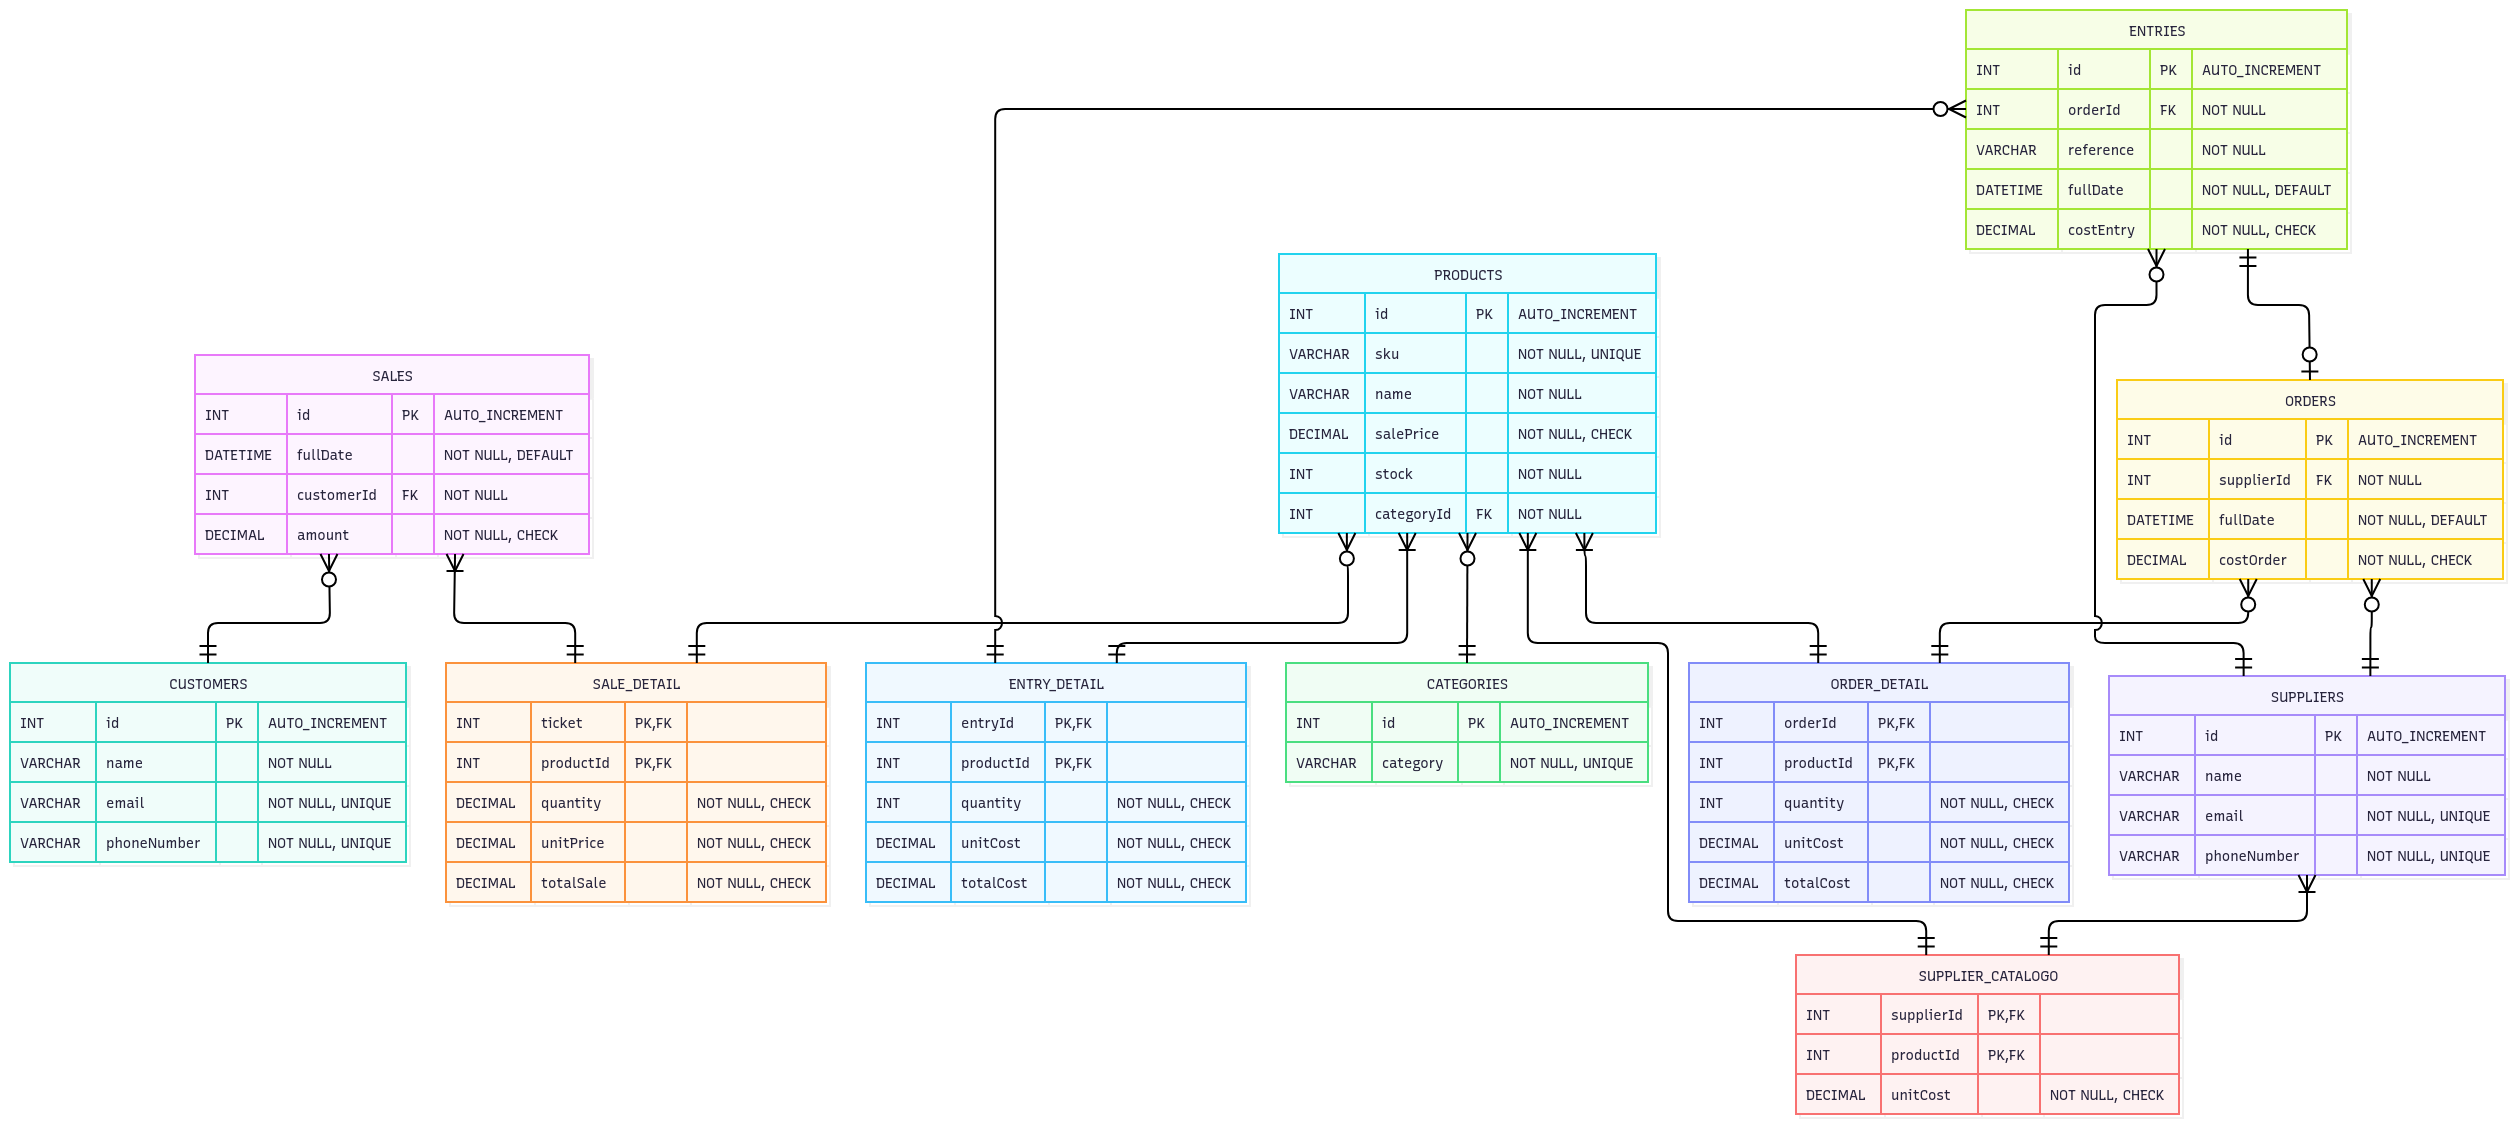
\includegraphics[
        width=0.7\textheight,
        height=0.7\textwidth,
        angle=-90
        ]{../img/relationalModel.drawio.png}
	\caption{Modelo relacional}
	\label{fig:relationalModel}
\end{figure}
\vfill
\newpage

\section*{\centering Diccionario de datos}
\addcontentsline{toc}{section}{Diccionario de datos}


\begin{table}
\centering
\begin{tabular}{&p{0.22\textwidth}&p{0.50\textwidth}&p{0.14\textwidth}&p{0.14\textwidth}&}
	\hline
	\textbf{Tabla} & \textbf{Descripción} & \textbf{Clave(s) primarias(s)} & \textbf{Clave(s) foránea(s)} \\
    \hline
    \texttt{PRODUCTS}            & Los artículos que vende una tienda, que adquiere el cliente y fabrica o distribuye un proveedor.      & \texttt{id}                               & \texttt{categoryId} \\
    \hline
    \texttt{SUPPLIERS}           & Los agentes que entregan la mercancía a la tienda para que este lo distribuya y venda.                & \texttt{id}                               & \\
    \hline
    \texttt{ENTRIES}             & El proceso de una tienda de recibir la mercancía al proveedor.                                        & \texttt{id}                               & \texttt{orderId} \\
    \hline
    \texttt{ORDERS}              & El proceso de una tienda de solicitar resurtido de mercancía al proveedor.                            & \texttt{id}                               & \texttt{supplierId} \\
    \hline
    \texttt{SALES}               & Las transacciones entre clientes y la tienda, donde el primero adquiere un artículo usando su dinero. & \texttt{id}                               & \texttt{customerId} \\
    \hline
    \texttt{CUSTOMERS}           & Los agentes que adquiere los productos ofertados por la tienda.                                       & \texttt{id}                               & \\
    \hline
    \texttt{CATEGORIES}          & La clasificación de la mercancía según su utilidad, caducidad u otros criterios.                      & \texttt{id}                               & \\
    \hline
    \texttt{SUPPLIER\_CATALOGO}  & Los productos ofertados por los proveedores.                                                          & \texttt{supplierId}, \texttt{productId}   & \texttt{supplierId}, \texttt{productId} \\
    \hline
    \texttt{ENTRY\_DETAIL}       & El desglose de mercancía recibida de un proveedor.                                                    & \texttt{entryId}, \texttt{productId}      &  \texttt{entryId}, \texttt{productId} \\
    \hline
    \texttt{ORDER\_DETAIL}       & El desglose de mercancía solicitada a un proveedor.                                                   & \texttt{orderid}, \texttt{productId}      & \texttt{orderid}, \texttt{productId} \\
    \hline
    \texttt{SALE\_DETAIL}        & El desglose de una venta, los productos y precios vendidos a un cliente.                              & \texttt{ticket}, \texttt{productId}       & \texttt{ticket}, \texttt{productId} \\
    \hline
\end{tabular}
\caption{Diccionario de datos por entidad}
\label{tab:diccionario-entidad}
\end{table}

\begin{table}
\centering
\begin{tabular}{cccccc}
    \textbf{Tabla} & \textbf{Columna} & \textbf{Tipo} & \textbf{Longitud o precisión} & \textbf{Nulo} & \textbf{Clave} & \textbf{Valor por defecto} & \textbf{Restricciones} & \textbf{Descripción} \\
    PRODUCTS          & id          & INT       &                      & No   & PK                                  & AUTO_INCREMENT    &               & Identificador único de producto. \\
    PRODUCTS          & sku         & VARCHAR   & 30                   & No   &                                     &                   & UNIQUE        & Código EAN-13 u otros de producto. \\
    PRODUCTS          & name        & VARCHAR   & 50                   & No   &                                     &                   &               & Nombre descriptivo del producto. \\
    PRODUCTS          & salePrice   & DECIMAL   & (10, 2)              & No   &                                     &                   & CHECK >= 0    & Precio de venta. \\
    PRODUCTS          & stock       & INT       &                      & No   &                                     &                   &               & Existencias del producto. \\
    PRODUCTS          & categoryId  & INT       &                      & No   & FK \longrightarrow CATEGORIES       &                   &               & Categoría única del producto. \\
    SUPPLIERS         & id          & INT       &                      & No   & PK                                  & AUTO_INCREMENT    &               & Identificador único de proveedor. \\
    SUPPLIERS         & name        & VARCHAR   & 50                   & No   &                                     &                   &               & Nombre o razón social del proveedor. \\
    SUPPLIERS         & email       & VARCHAR   & 50                   & No   &                                     &                   & UNIQUE        & Correo electrónico del proveedor. \\
    SUPPLIERS         & phoneNumber & VARCHAR   & 20                   & No   &                                     &                   & UNIQUE        & Número telefónico del proveedor. \\
    ENTRIES           & id          & INT       &                      & No   & PK                                  & AUTO_INCREMENT    &               & Identificador único de recepción de mercancía. \\
    ENTRIES           & orderId     & INT       &                      & No   & FK \longrightarrow ORDERS           &                   &               & Identificador de pedido. \\  
    ENTRIES           & reference   & VARCHAR   & 36                   & No   &                                     &                   &               & Nota de venta o factura entregada por el proveedor. \\
    ENTRIES           & fullDate    & DATETIME  &                      & No   &                                     & CURRENT_TIMESTAMP &               & Fecha y hora de recepción. \\
    ENTRIES           & costEntry   & DECIMAL   & (10, 2)              & No   &                                     &                   & CHECK >= 0    & Costo total de la recepción. \\
    ORDERS            & id          & INT       &                      & No   & PK                                  & AUTO_INCREMENT    &               & Identificador único de pedido de mercancía. \\
    ORDERS            & supplierId  & INT       &                      & No   & FK \longrightarrow SUPPLIERS        &                   &               & Identificador de proveedor. \\
    ORDERS            & fullDate    & DATETIME  &                      & No   &                                     & CURRENT_TIMESTAMP &               & Fecha y hora de solicitud de pedido. \\
    ORDERS            & costOrder   & DECIMAL   & (10, 2)              & No   &                                     &                   & CHECK >= 0    & Costo total del pedido. \\    
    SALES             & id          & INT       &                      & No   & PK                                  & AUTO_INCREMENT    &               & Identificador único de venta. \\
    SALES             & fullDate    & DATETIME  &                      & No   &                                     &                   &               & Fecha y hora de la venta. \\
    SALES             & customerId  & INT       &                      & No   & FK \longrightarrow CUSTOMERS        & CURRENT_TIMESTAMP &               & Cliente vinculado a la compra. \\
    SALES             & amount      & DECIMAL   & (10,2)               & No   &                                     &                   & CHECK >= 0    & Monto total de la venta. \\      
    CUSTOMERS         & id          & INT       &                      & No   & PK                                  & AUTO_INCREMENT    &               & Identificador único de cliente. \\
    CUSTOMERS         & name        & VARCHAR   & 50                   & No   &                                     &                   &               & Nombre del cliente. \\             
    CUSTOMERS         & email       & VARCHAR   & 50                   & No   &                                     &                   & UNIQUE        & Correo electrónico del cliente. \\ 
    CUSTOMERS         & phoneNumber & VARCHAR   & 20                   & No   &                                     &                   & UNIQUE        & Número telefónico del cliente. \\  
    CATEGORIES        & id          & INT       &                      & No   & PK                                  & AUTO_INCREMENT    &               & Identificador único de categoría. \\   
    CATEGORIES        & category    & VARCHAR   & 50                   & No   &                                     &                   & UNIQUE        & Nombre descriptivo de la categoría. \\ 
    SUPPLIER_CATALOGO & supplierId  & INT       &                      & No   & PK, FK \longrightarrow SUPPLIERS    &                   &               & Identificador de proveedor. \\                    
    SUPPLIER_CATALOGO & productId   & INT       &                      & No   & PK, FK \longrightarrow PRODUCTS     &                   &               & Identificador de producto. \\                     
    SUPPLIER_CATALOGO & unitCost    & DECIMAL   & (10,2)               & No   &                                     &                   & CHECK >= 0    & Costo unitario, precio proveedor del producto. \\ 
    ENTRY_DETAIL      & entryId     & INT       &                      & No   & PK, FK \longrightarrow ENTRIES      &                   &               & Identificador de recepción de mercancía. \\      
    ENTRY_DETAIL      & productId   & INT       &                      & No   & PK, FK \longrightarrow PRODUCTS     &                   &               & Identificador de producto. \\                    
    ENTRY_DETAIL      & quantity    & INT       &                      & No   &                                     &                   & CHECK >= 0    & Cantidad recibida de producto. \\                
    ENTRY_DETAIL      & unitCost    & DECIMAL   & (10,2)               & No   &                                     &                   & CHECK >= 0    & Costo unitario de producto, precio proveedor.  \\
    ENTRY_DETAIL      & totalCost   & DECIMAL   & (10,2)               & No   &                                     &                   & CHECK >= 0    & Costo total por producto.  \\
    ORDER_DETAIL      & orderId     & INT       &                      & No   & PK, FK \longrightarrow ORDERS       &                   &               & Identificador de pedido de mercancía.  \\
    ORDER_DETAIL      & productId   & INT       &                      & No   & PK, FK \longrightarrow PRODUCTS     &                   &               & Identificador de producto. \\           
    ORDER_DETAIL      & quantity    & INT       &                      & No   &                                     &                   & CHECK >= 0    & Cantidad solicitada de producto. \\
    ORDER_DETAIL      & unitCost    & DECIMAL   & (10,2)               & No   &                                     &                   & CHECK >= 0    & Costo unitario de producto, precio proveedor. \\
    ORDER_DETAIL      & totalCost   & DECIMAL   & (10,2)               & No   &                                     &                   & CHECK >= 0    & Costo total por producto. \\                    
    SALE_DETAIL       & ticket      & INT       &                      & No   & PK, FK \longrightarrow ORDERS       &                   &               & Identificador de venta. \\                  
    SALE_DETAIL       & productId   & INT       &                      & No   & PK, FK \longrightarrow PRODUCTS     &                   &               & Identificador de producto. \\               
    SALE_DETAIL       & quantity    & INT       &                      & No   &                                     &                   & CHECK >= 0    & Cantidad vendida de producto. \\
    SALE_DETAIL       & unitPrice   & DECIMAL   & (10,2)               & No   &                                     &                   & CHECK >= 0    & Precio unitario, precio de venta del producto. \\
    SALE_DETAIL       & totalSale   & DECIMAL   & (10,2)               & No   &                                     &                   & CHECK >= 0    & Monto total de venta. \\                  
\end{tabular}
\caption{Diccionario de datos por atributo}
\label{tab:diccionario-atributo}
\end{table}{}

\section*{}
\addcontentsline{toc}{section}{}


% \begin{figure}[h!]
% 	\centering
% 	\begin{subfigure}[b]{0.45\linewidth}
% 		\includegraphics[width=\linewidth]{./img/bd-json.png}
% 		\caption{Orientado a documentos}
% 		\label{fig:bd-json}
% 	\end{subfigure}
% 	\begin{subfigure}[b]{0.295\linewidth}
% 		\includegraphics[width=\linewidth]{./img/bd-objetos.png}
% 		\caption{Orientado a objetos}
% 		\label{fig:bd-objeto}
% 	\end{subfigure}
% 	\caption{Base de datos no relacionales}
% 	\label{fig:base-nosql}
% \end{figure}

\section*{Conclusión}
\addcontentsline{toc}{section}{Conclusión}



\listoftables
\listoffigures

\end{document}